\section{Plotting Bivariate Data in R}


Let's use a dataset called |iris| (included in the standard R distribution) to explore bivariate relationships between variables. This data set was made famous by R. A. Fisher who used it to illustrate many of the fundamental statistical methods he developed. The data set consists of four morphometric measurements on specimens of three different iris species. Use the R help to read about the iris data set (\lstinline!?iris!). We'll be using this data set repeatedly in future weeks so familiarize yourself with it.
%
\begin{R}
> ?iris
> names(iris)
[1] "Sepal.Length" "Sepal.Width"  "Petal.Length" "Petal.Width"
[5] "Species"
> unique(iris$Species)
[1] setosa     versicolor virginica
Levels: setosa versicolor virginica
> dim(iris)
[1] 150   5
\end{R}


\subsection{Bivariate scatter plots}
We'll start with the conventional `variable space' representation of bivariate relationships -- the scatter plot.
%
\begin{R}
> plot(iris$Sepal.Length, iris$Sepal.Width)
\end{R}
%
This plots Sepal Length on the x-axis and Petal Length on the y-axis. Here's an alternate way to generate the same plot:
%
\begin{R}
> plot(Petal.Length ~ Sepal.Length, data = iris)
\end{R}
%
Did you notice what is different between the two versions above?  In the second version, you can think of the tilde (`~') as short-hand for `function of'.  So the plotting call above can be translated roughly as ``Plot Petal.Length as a function of Sepal.Length, where these variables can be found in the iris data set''.

From these plot it is immediately obvious that these two variables are positively associated (i.e. when one increases the other tends to increase). You will also notice there seem to be distinct clusters of points in the plot. Recall that the iris data set consists of three different species.  Let's regenerate the plot, this time coloring the points according to the species names.
%
First, let's note that the Species column is a categorical variable, which in R we refer to as a `factor'.
%
\begin{R}
> iris$Species
  [1] setosa     setosa     setosa     setosa ...    
 [51] versicolor versicolor versicolor versicolor ...
[101] virginica  virginica  virginica  virginica  ...
  ....
Levels: setosa versicolor virginica
> is.factor(iris$Species)
[1] TRUE
> levels(iris$Species)
[1] "setosa"     "versicolor" "virginica" 
> nlevels(iris$Species)
[1] 3
> typeof(iris$Species)
[1] "integer"
\end{R}
The |is.factor()| function tests whether an vector is a factor,  the |levels()| function returns the categorical labels associated with the factor, and |nlevels()| gives the total number of levels. Factor levels are represented internally as integers, as the |typeof()| function call illustrates.  You can use the function |unclass()| to show the corresponding integer representations for a vector of factors:
%
\begin{R}
> unclass(iris$Species)
  [1] 1 1 1 1 1 1 1 1 1 1 1 1 1 1 1 1 1 1 1 1 1 1 ...
 [59] 2 2 2 2 2 2 2 2 2 2 2 2 2 2 2 2 2 2 2 2 2 2 ...
[117] 3 3 3 3 3 3 3 3 3 3 3 3 3 3 3 3 3 3 3 3 3 3 ...
attr(,"levels")
[1] "setosa"     "versicolor" "virginica" 
\end{R}
%
As you can see, the `setosa' specimens have the value 1, `versicolor' have the value 2, and `virginica' the value 3.

Because of the mapping between factor levels and integers, we can use a variable of factors as indices into another vector, effectively creating a mapping between the factor levels, and the elements of the vector that is being indexed.  This is shown below:
\begin{R}
> clrs <- c('red','green','blue')
> clrs[iris$Species]
  [1] "red"   "red"   "red"   "red"   "red"   "red"   "red" ...
 [57] "green" "green" "green" "green" "green" "green" "green" ...
 [99] "green" "green" "blue"  "blue"  "blue"  "blue"  "blue" ...
\end{R}
%
With that mapping in mind, let's reconstruct our scatter plot:
\begin{R}
> plot(Petal.Length ~ Sepal.Length, data = iris, col = clrs[iris$Species], main="Petal Length vs. Sepal Length")
> legend( "topleft", pch = 1, col = clrs, legend = levels(iris$Species ))
\end{R}
%
In addition to plotting and coloring the bivariate scatter, we added a title to the plot using the |main| argument and created a legend, using the |legend()| function.  Your output should look like Figure~\ref{fig:irisscatter}.
%
\begin{figure}[htbp]
\centering
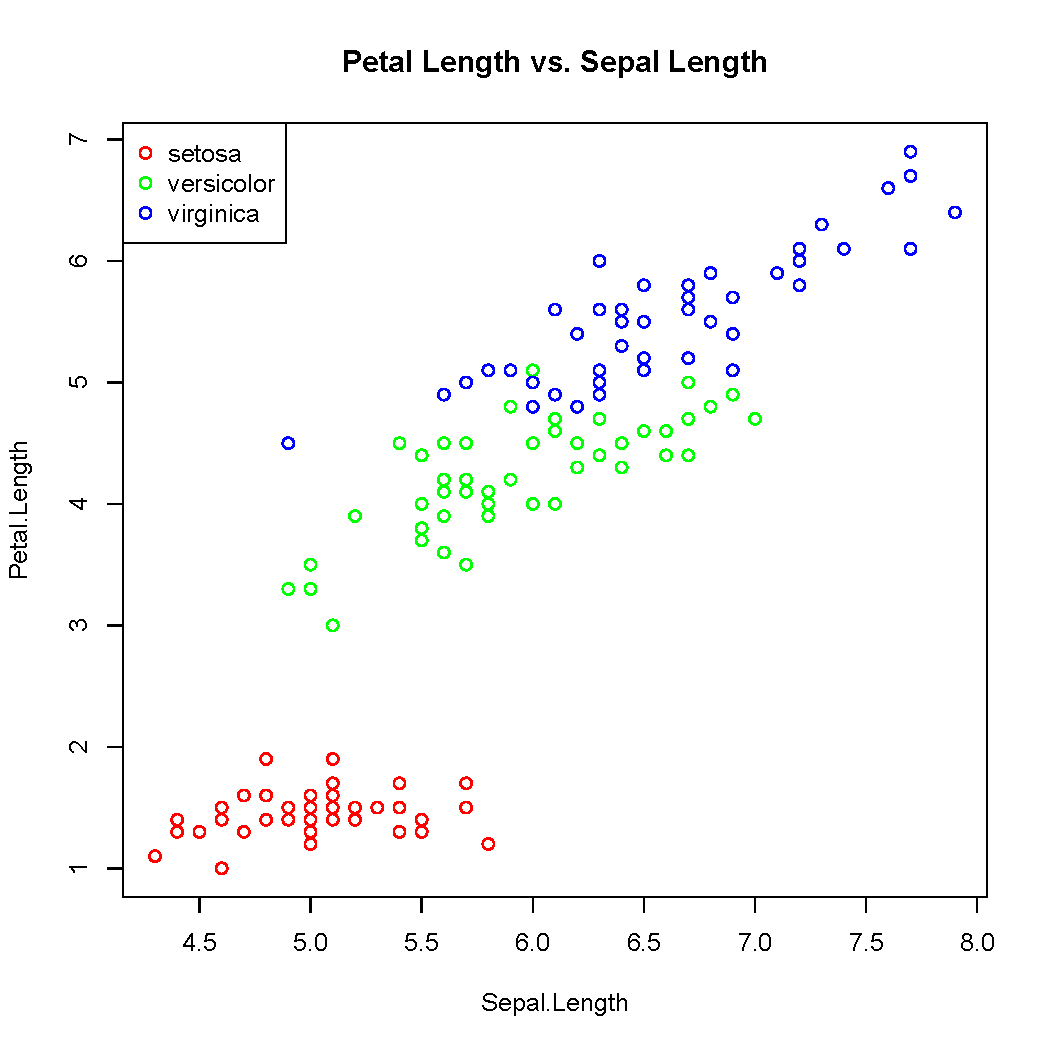
\includegraphics[width=0.4\columnwidth]{./figures/hands-on2/iris-scatter.pdf}
\caption{Scatter plot created from the iris data set using the \lstinline!plot! function.}
\label{fig:irisscatter}
\end{figure}


